\begin{center}
    \Large{\textbf{Практична частина}}
\end{center}

\vspace{1mm}

У результаті проведених експериментів отримані наступні дослідні дані.
\begin{table}[h]
    \centering
    \begin{tabular}{|c|c|c|}
        \hline
        \textbf{L(см)} & \textbf{Номер кільця} & \textbf{r(см)} \\
        \hline

        \multirow{10}{*}{60} & 1 & 1 \\
        \cline{2-3}
        & 2 & 1.35 \\
        \cline{2-3}
        & 3 & 1.6 \\        
        \cline{2-3}
        & 4 & 1.8 \\
        \cline{2-3}
        & 5 & 2 \\        
        \cline{2-3}
        & 6 & 2.2  \\
        \cline{2-3}
        & 7 & 2.4  \\
        \cline{2-3}        
        & 8 & 2.55  \\
        \cline{2-3}
        & 9 & 2.7  \\
        \cline{2-3}        
        & 10 & 2.85  \\
        \hline
        
        \multirow{10}{*}{80} & 1 & 1.4  \\
        \cline{2-3}
        & 2 & 1.8 \\
        \cline{2-3}
        & 3 & 2.2 \\        
        \cline{2-3}
        & 4 & 2.5 \\
        \cline{2-3}
        & 5 & 2.8 \\        
        \cline{2-3}
        & 6 & 3 \\
        \cline{2-3}
        & 7 & 3.25 \\
        \cline{2-3}        
        & 8 & 3.5 \\
        \cline{2-3}
        & 9 & 3.65 \\
        \cline{2-3}        
        & 10 & 3.85 \\
        \hline

        \multirow{10}{*}{100} & 1 & 1.6 \\
        \cline{2-3}
        & 2 & 2.2 \\
        \cline{2-3}
        & 3 & 2.7 \\        
        \cline{2-3}
        & 4 & 3.05 \\
        \cline{2-3}
        & 5 & 3.4 \\        
        \cline{2-3}
        & 6 & 3.75 \\
        \cline{2-3}
        & 7 & 4.05 \\
        \cline{2-3}        
        & 8 & 4.35 \\
        \cline{2-3}
        & 9 & 4.6 \\
        \cline{2-3}        
        & 10 & 4.75 \\
        \hline

    \end{tabular}
    \caption{Дослідні дані}
\end{table}

\begin{figure}[h!]
    Обрахуємо значення $B$ та $\Theta$
    $$ B_i = r_{i+1} - r_i $$
    $$ \Theta_i = \frac{ r_i }{2L} $$
\end{figure}

\begin{table}[h]
    \centering
    \begin{tabular}{|c|c|c|c|c|c|c|c|c|c|}
        \hline
        \textbf{L} & $B_1$ & $B_2$ & $B_3$ & $B_4$ & $B_5$ & $B_6$ & $B_7$ & $B_8$ & $B_9$ \\
        \hline
        60 & 0.35 & 0.25 & 0.2 & 0.2 & 0.2 & 0.2 & 0.15 & 0.15 & 0.15 \\
        \hline
        80 & 0.4 & 0.4 & 0.3 & 0.3 & 0.2 & 0.25 & 0.25 & 0.15 & 0.2 \\
        \hline
        100 & 0.6 & 0.5 & 0.35 & 0.35 & 0.35 & 0.3 & 0.3 & 0.25 & 0.15 \\
        \hline
    \end{tabular}
    
    \caption{Результати обрахунку $B$}
\end{table}

\begin{table}[h!]
    \centering
    \begin{tabular}{|c|c|c|c|c|c|c|c|c|c|}
        \hline
        \textbf{L} & $\Theta_1$ & $\Theta_2$ & $\Theta_3$ & $\Theta_4$ & $\Theta_5$ & $\Theta_6$ & $\Theta_7$ & $\Theta_8$ & $\Theta_9$ \\
        \hline
        60 & 0.008 & 0.011 & 0.013 & 0.015 & 0.017 & 0.018 & 0.02 & 0.021 & 0.023 \\
        \hline
        80 & 0.009 & 0.011 & 0.014 & 0.016 & 0.018 & 0.019 & 0.02 & 0.022 & 0.23 \\
        \hline
        100 & 0.008 & 0.011 & 0.014 & 0.015 & 0.017 & 0.019 & 0.02 & 0.22 & 0.023 \\
        \hline
    \end{tabular}
    
    \caption{Результати обрахунку $\Theta$}
\end{table}

\begin{table}[h!]
    \centering
    \begin{tabular}{|c|c|c|c|c|c|c|c|c|c|}
        \hline
        \textbf{L} & $B\Theta_1$ & $B\Theta_2$ & $B\Theta_3$ & $B\Theta_4$ & $B\Theta_5$ & $B\Theta_6$ & $B\Theta_7$ & $B\Theta_8$ & $B\Theta_9$ \\
        \hline
        60 & 0.0029 & 0.0028 & 0.0027 & 0.003 & 0.0033 & 0.0037 & 0.003 & 0.0032 & 0.0034 \\
        \hline
        80 & 0.0035 & 0.0045 & 0.0041 & 0.0047 & 0.0035 & 0.0047 & 0.0051 & 0.0033 & 0.0046 \\
        \hline
        100 & 0.0045 & 0.0055 & 0.0047 & 0.0053 & 0.006 & 0.00556 & 0.006 & 0.0054 & 0.0034 \\
        \hline
    \end{tabular}
    
    \caption{Результати обрахунку $B\Theta$}
\end{table}

\begin{figure}[h!]
    Апроксимуємо залежність $B\Theta(L)$ лінійною функцією $B\Theta = k L + b$
    Графік отриманою залежності наведено нижче.
\end{figure}

\begin{figure}[h!]    
    \centering
    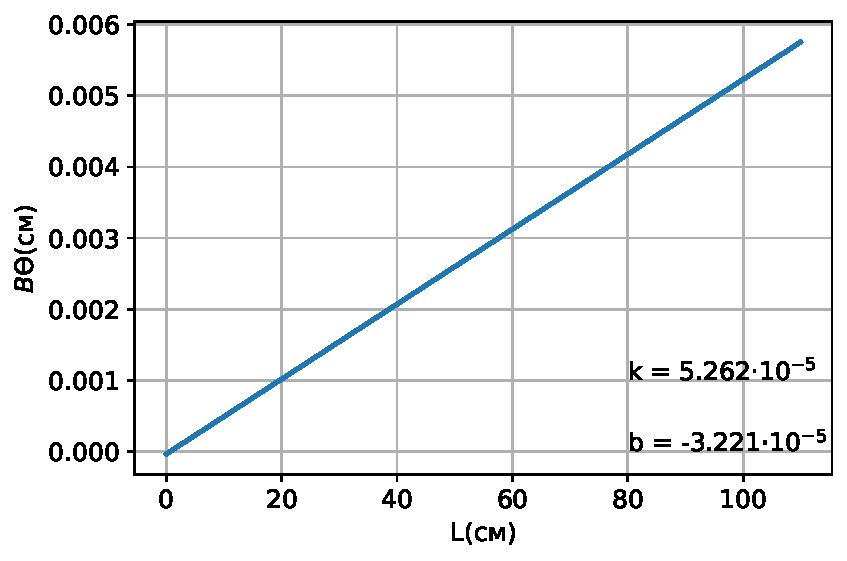
\includegraphics[width=.6\textwidth]{assets/BQ(l).pdf}
    \caption{Графік залежності $B\Theta(L)$}
\end{figure}


\begin{figure}[h!]
    З формули \ref{eq:2} слідує, що показник заломлення дорівнює($h_0 = 16.25*10^{-1}$(см))
    $$ n = \frac{kh_0}{\lambda} \simeq 1.35 $$
\end{figure}
